\iffalse
\chapter{2022}
\author{AI24BTECH11022}
\section{ee}
\fi

\item An inductor having a $Q-$Factor of $60$ is connected in series with a capacitor having a $Q-$factor of $240$. The overall $Q-$factor of the circuit is \rule{1cm}{0.15mm} (round off to nearest integer)\hfill(2022)


\item The network shown below has a resonant frequency of $150kHz$ and a bandwidth of $600Hz$. The $Q-$factor of the network is \rule{1cm}{0.15mm} (round off to nearest integer)\hfill(2022)

\begin{circuitikz}
\draw (4,0) to [R=$R$] (4,2) to [L=$L$] (4,4) -- (0,4);
\draw (4,0) -- (0,0);
\draw (2,0) to [C=$C$] ++(0,4);
\end{circuitikz}


\item The maximum clock frequency in $MHz$ of a $4-$stage ripple counter, utilizing flip-flops, with each flip-flop having a propagation delay of $20ns$, is \rule{1cm}{0.15mm}. (round off to one decimal place)\hfill(2022)


\item If only $5\%$ of the supplied power to a cable reaches the output terminal, the power loss in the cable, in $decibels$, is \rule{1cm}{0.15mm}. (round off to nearest integer)\hfill(2022)


\item In the circuit shown below, the switch $S$ is closed at $t=0$. The magnitude of the steady state voltage, in $volts$, across the $6\ohm$ resistor is \rule{1cm}{0.15mm}. (round off to two decimal places)\hfill(2022)

\begin{circuitikz}
\draw (5,0) to [R=$2\ohm$] (3,0) to [closing switch, l=S] (2,0) to [battery1,l=$10V$] (0,0) -- (0,1) to [C=$1\mu F$] (2.5,1) to [R=$10\ohm$] (5,1);
\draw (4,3) -- (5,3) -- (5,0);
\draw (0,0) -- (0,3) -- (1,3) -- (1,3.5) to [R=$6\ohm$] (4,3.5) -- (4,2.5) to [R=$3\ohm$] (1,2.5) -- (1,3);
\end{circuitikz}


\item A single-phase full-bridge diode rectifier feeds a resistive load of $50\ohm$ from a $200V$, $50Hz$ single phase $AC$ supply. If the diodes are ideal, then the active power, in $watts$, drawn by the load is \rule{1cm}{0.15mm}. (round off to nearest integer)\hfill(2022)


\item The voltage at the input of an AC-DC rectifier is given by $v\brak{t}=230\sqrt{2}sin{\omega t}$ where $\omega=2\pi\times 50rad/s$. The input current drawn by the rectifier is given by $$i\brak{t}=10\sin{\brak{\omega t-\frac{\pi}{3}}}+4\sin{\brak{3\omega t-\frac{\pi}{6}}}+3\sin{\brak{5\omega t-\frac{\pi}{3}}}$$ The input power factor, (rounded off to two decimal places), is, \rule{1cm}{0.15mm} lag.\hfill(2022)


\item Two balanced three-phase loads, as shown in the figure, are connected to a $100\sqrt{3}V$, three-phase, $50Hz$ main supply Given $Z_{1}=(18+j24)\ohm$ and $Z_{2}=\brak{6+j8}\ohm$. The ammeter reading, in amperes, is \rule{1cm}{0.15mm}. (round off to nearest integer)\hfill(2022)

\begin{circuitikz}[scale=0.25]
\draw node[left] {$B$} (0,0) -- (25,0) to [generic,l=$Z_{1}$] (25,20) to [generic,l=$Z_{2}$] (17.5,10) to [generic,l=$Z_{2}$] (25,0) to [generic,l=$Z_{1}$] (5,10) to [generic,l=$Z_{1}$] (25,20) -- (8.5,20);
\draw (6.5,20) --  (0,20) node[left] {$R$};
\draw (7.5,20) circle (1cm);
\draw (17.5,10) to [generic,l=$Z_{2}$] (10,10) -- (0,10) node[left] {$Y$};
\node at (7.5,20) {$A$};
\filldraw (17.5,10) circle (0.5cm);
\draw[<->] (2,10) -- (2,20) node[midway,left] {$100\sqrt{3}V$};
\end{circuitikz}


\item The frequencies of the stator and rotor currents flowing in a three-phase $8-$pole induction motor are $40Hz$ and $1Hz$, respectively. The motor speed, in rpm, is \rule{1cm}{0.15mm}. (round off to nearest integer)\hfill(2022)


\item The output impedance of a non-ideal operational amplifier is denoted by $Z_{out}$. The variation in the magnitude of $Z_{out}$ with increasing frequency, $f$, in the circuit shown below, is best represented by\hfill(2022)

\begin{circuitikz}
\draw (2,2) node[op amp] (opamp) {};
\draw (0,0) to[sV, l=$V_{\text{in}}$] (0,1.5) -- (opamp.+);
\draw (opamp.-) |- (1,3.5) -| (opamp.out);
\draw (opamp.out) -- ++(1,0) node[right] {$V_{\text{out}}$};
\draw (0,0) -- (0,-0.1) node[ground] {};
\end{circuitikz}
\begin{multicols}{2}
\begin{enumerate}
\item 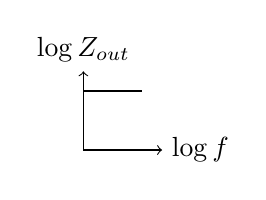
\begin{tikzpicture}
\draw[->] (0,0) -- (1,0) node[right] {$\log\brak{f}$};
\draw[->] (0,0) -- (0,1) node[above] {$\log\brak{\abs{Z_{out}}}$};
\draw (0,0.75) -- (0.75,0.75);
\end{tikzpicture}
\item 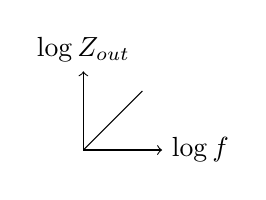
\begin{tikzpicture}
\draw[->] (0,0) -- (1,0) node[right] {$\log\brak{f}$};
\draw[->] (0,0) -- (0,1) node[above] {$\log\brak{\abs{Z_{out}}}$};
\draw (0,0) -- (0.75,0.75);
\end{tikzpicture}
\item 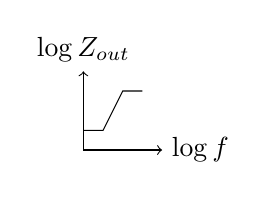
\begin{tikzpicture}
\draw[->] (0,0) -- (1,0) node[right] {$\log\brak{f}$};
\draw[->] (0,0) -- (0,1) node[above] {$\log\brak{\abs{Z_{out}}}$};
\draw (0,0.25) -- (0.25,0.25) -- (0.5,0.75) -- (0.75,0.75);
\end{tikzpicture}
\item 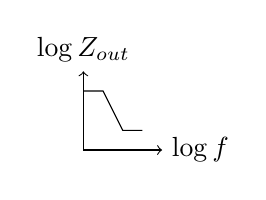
\begin{tikzpicture}
\draw[->] (0,0) -- (1,0) node[right] {$\log\brak{f}$};
\draw[->] (0,0) -- (0,1) node[above] {$\log\brak{\abs{Z_{out}}}$};
\draw (0,0.75) -- (0.25,0.75) -- (0.5,0.25) -- (0.75,0.25);
\end{tikzpicture}
\end{enumerate}
\end{multicols}


\item An $LTI$ system is shown in the figure where $G\brak{s}=\frac{100}{s^{2}+0.1s+10}$. The steady state output of the system, to the input $r\brak{t}$, is given as $y\brak{t}=a+b\sin{\brak{10t+\theta}}$. The values of '$a$' and '$b$' will be\hfill(2022)

\begin{tikzpicture}
\draw[->] (0,1) -- (1,1);
\draw (1,1) -- (2,1);
\draw (2,0) rectangle (5,2);
\draw[->] (5,1) -- (6,1);
\draw (6,1) -- (7,1);
\node[above] at (0,1) {$r\brak{t}=1+0.1\sin{\brak{10t}}$};
\node[above] at (6,1) {$y\brak{t}$};
\node at (3.5,1) {$G\brak{s}$};
\end{tikzpicture}
\begin{multicols}{2}
\begin{enumerate}
\item $a=1$, $b=10$
\item $a=10$, $b=1$
\item $a=1$, $b=100$
\item $a=100$, $b=1$
\end{enumerate}
\end{multicols}


\item The open loop transfer function of a unity gain negative feedback system is given as $G\brak{s}=\frac{1}{s\brak{s+1}}$. The Nyquist contour in the $s-$plane encloses the entire right half plane and a small neighbourhood around the origin in the left half plane, as shown in the figure below. The number of encirclements of the point $\brak{-1+j0}$ by the Nyquist plot of $G\brak{s}$, corresponding to the Nyquist contour, is denoted as $N$. Then $N$ equals to\hfill(2022)

\begin{tikzpicture}[scale=2]
\draw (-1,0) -- (1,0);
\draw (0,-1) -- (0,1);
\node[below] at (1.5,0) {$\rightarrow Re\brak{s}$};
\node[left] at (0,1) {$Im\brak{s}\uparrow$};
\draw[->] (0,2/3) arc[start angle=90,end angle=0,radius=2/3];
\draw[->] (2/3,0) arc[start angle=0,end angle=-90,radius=2/3];
\draw[->] (0,-1) -- (0,-0.4);
\draw[->] (0,-1/3) arc[start angle=-90,end angle=-180,radius=1/3];
\draw[->] (-1/3,0) arc[start angle=180,end angle=90,radius=1/3];
\draw[->] (0,1/3) -- (0,0.55);
\end{tikzpicture}
\begin{multicols}{2}
\begin{enumerate}
\item $0$
\item $1$
\item $2$
\item $3$
\end{enumerate}
\end{multicols}


\item The damping ratio and undamped natural frequency of a closed loop system as shown in the figure, are denoted as $\zeta$ and $w_{n}$, respectively. The values of $\zeta$ and $w_{n}$ are\hfill(2022)

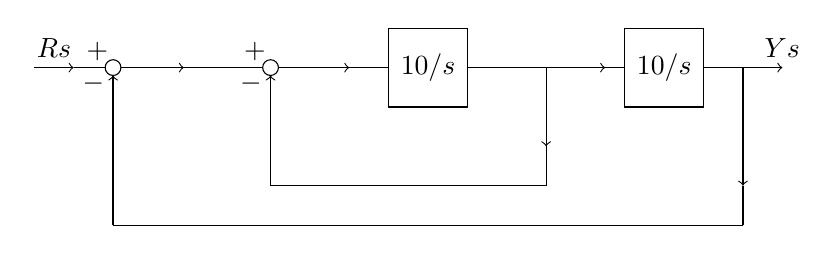
\begin{tikzpicture}
\draw[->] (0,3) -- (0.5,3) node[midway,above] {$R\brak{s}$};
\draw (0.5,3) -- (0.9,3);
\draw[->] (1.1,3) -- (1.9,3);
\draw (1.9,3) -- (2.9,3);
\draw[->] (3.1,3) -- (4,3);
\draw (3.5,3) -- (4.5,3);
\draw (4.5,2.5) rectangle (5.5,3.5);
\draw[->] (5.5,3) -- (7.25,3);
\draw (7,3) -- (7.5,3);
\draw (7.5,2.5) rectangle (8.5,3.5);
\draw[->] (8.5,3) -- (9.5,3) node[right,above] {$Y\brak{s}$};
\draw (1,3) circle (0.1cm);
\draw (3,3) circle (0.1cm);
\draw[->] (6.5,3) -- (6.5,2);
\draw (6.5,2) -- (6.5,1.5);
\draw (6.5,1.5) -- (3,1.5);
\draw[->] (3,1.5) -- (3,2.9);
\draw[->] (9,3) -- (9,1.5);
\draw (9,1.5) -- (9,1);
\draw (9,1) -- (1,1);
\draw[->] (1,1) -- (1,2.9);
\node at (5,3) {$10/s$};
\node at (8,3) {$10/s$};
\node at (0.8,3.2) {$+$};
\node at (0.75,2.8) {$-$};
\node at (2.8,3.2) {$+$};
\node at (2.75,2.8) {$-$};
\end{tikzpicture}
\begin{multicols}{2}
\begin{enumerate}
\item $\zeta=0.5$ and $w_{n}=10rad/s$
\item $\zeta=0.1$ and $w_{n}=10rad/s$
\item $\zeta=0.707$ and $w_{n}=10rad/s$
\item $\zeta=0.707$ and $w_{n}=100rad/s$
\end{enumerate}
\end{multicols}